\pdfminorversion=4
\documentclass{beamer}
\usepackage[ngerman]{babel}
\usepackage[utf8]{inputenc}
\usepackage{graphicx}
\usetheme{Warsaw}
\title{Mit Kryptographie die Welt retten}
\subtitle{Cypherpunk in Theorie und Praxis}
\author{Sebastian Beschke \\ \texttt{sebastian@sbeschke.de}}
\institute{Chaostreff Tübingen}
\date{01. 10. 2011}
\begin{document}

\begin{frame}
\titlepage
\end{frame}


\begin{frame}
	\frametitle{Überblick}
	\tableofcontents
\end{frame}

\section{Einführung in die Public-Key-Kryptographie}
\subsection{Geheimschrift}

\begin{frame}
\frametitle{Eine einfache Chiffre}
\begin{columns}

\column{0.5\textwidth}
	\texttt{FBSKHUSXQNV ZULWH FRGH}

\pause	\texttt{cypherpunks write code}

\column{0.5\textwidth}
\pause	\(K=3\)

	\textit{Schlüssel}

\end{columns}
\end{frame}

\begin{frame}
\frametitle{Symmetrische und Public-Key-Verschlüsselung}
\begin{columns}

\column{0.5\textwidth}
	\textbf{Symmetrisches Verfahren:}
	
	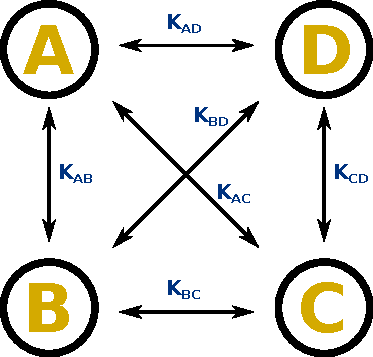
\includegraphics[width=0.9\textwidth]{images/symmetric.pdf}\\

	\small{Verschlüsselung und Entschlüsselung mit gleichem Schlüssel}

	\(\frac{n(n-1)}{2}\) Schlüssel

\pause
\column{0.5\textwidth}
	\textbf{Public-Key-Verfahren:}

	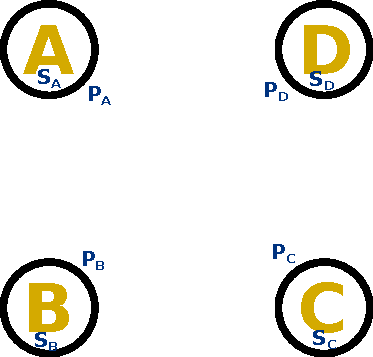
\includegraphics[width=0.9\textwidth]{images/asymmetric.pdf}\\

	\small{Verschlüsselung mit öffentlichem Schlüssel; Entschlüsselung mit privatem Schlüssel}

	\(2n\) Schlüssel

\end{columns}
\end{frame}

\subsection{Das RSA-Verfahren}

\begin{frame}
\frametitle{Das RSA-Verfahren}

	\begin{itemize}
		\item RSA ist eines der ältesten Public-Key-Verfahren (1978)
		\item Auch heute noch ein Standard-Verfahren
		\item Basiert auf der Modulo-Rechnung und dem Satz von Euler
		\item Deshalb jetzt ein wenig Mathe\dots
	\end{itemize}
\end{frame}

\begin{frame}
\frametitle{Modulo-Rechnung}
	\begin{itemize}
		\item Modulo-Rechnung ist das Rechnen mit Resten
		\item \(4 \cdot 4 \equiv \ ?\ (\text{mod}\ 5) \)
\pause		\item \(4 \cdot 4 = 16\)
\pause		\item \(16 : 5 = 3 \text{ Rest } \textbf{1}\)
\pause		\item Also \(4 \cdot 4 \equiv 1\ (\text{mod}\ 5) \)
	\end{itemize}
\end{frame}


\begin{frame}
\frametitle{Der Satz von Euler}

\begin{itemize}
	\begin{definition}[Die Eulersche \(\varphi\)-Funktion]
		\(\varphi(n) = \) Anzahl der zu \(n\) teilerfremden Zahlen \(\leq n\)
	\end{definition}
\pause	\item Ist \(p\) eine Primzahl, so ist \(\varphi(p) = p-1\)
	\item Ist \(n=pq\), \(p,q\) prim, so ist \(\varphi(n) = (p-1)(q-1)\)

\pause	\begin{theorem}[Der Satz von Euler]
		Seien \(a\) und \(n\) teilerfremd.
		Dann gilt \(a^{\varphi(n)} \equiv 1 \ (\text{mod}\ n)\)
	\end{theorem}
\end{itemize}
\end{frame}

\begin{frame}
\frametitle{Verschlüsseln mit dem Satz von Euler}

	\begin{theorem}[Der Satz von Euler]
		Seien \(a\) und \(n\) teilerfremd.
		Dann gilt \(a^{\varphi(n)} \equiv 1 \ (\text{mod}\ n)\)
	\end{theorem}

	\begin{itemize}
		\item Sei \(n\) das Produkt zweier Primzahlen \(p,q\)
		\item Angenommen, wir haben \(e,d\) mit \(ed = k \cdot \varphi(n) + 1\)
\pause		\item Sei \(m\) eine Nachricht.
		\item \(c \equiv m^e \ (\text{mod}\ n)\) ist dann die verschlüsselte Nachricht.
\pause		\item Kennt man \(d\), kann man sie entschlüsseln: \(c^d \equiv m^{ed} \equiv m^{k \cdot \varphi(n) + 1} \equiv m \cdot m^{k \cdot \varphi(n)} \equiv m \ (\text{mod}\ n)\)
	\end{itemize}
\end{frame}

\begin{frame}
\frametitle{RSA-Verschlüsselung}

\begin{itemize}
	\item \(n, e\) werden als öffentlicher Schlüssel veröffentlicht.
	\item \(p, q, d\) werden geheim gehalten.
	\item Jeder kann mit \(c \equiv m^e\ (\text{mod}\ n)\) verschlüsseln.
	\item Nur der Inhaber des geheimen Schlüssels kann mit \(m \equiv c^d \ (\text{mod}\ n)\) entschlüsseln.
\pause	\item Ein Angreifer könnte \(\log_e c\) berechnen.
	\begin{itemize}
		\item Das ist aber auf Restklassenringen sehr schwierig.
	\end{itemize}
\pause	\item Oder er könnte versuchen, \(d\) zu bestimmen.
	\begin{itemize}
		\item Der Knackpunkt: Zur Bestimmung von \(d\) braucht man \(\varphi(n)\)
		\item Leicht zu bestimmen, wenn man \(p,q\) kennt: \(\varphi(n)=(p-1)(q-1)\).
		\item Sonst aber sehr schwer zu bestimmen.
		\item RSA zu knacken, ist daher so schwer, wie die Primfaktorzerlegung von \(n\).
	\end{itemize}
\end{itemize}
\end{frame}

\section{Privatsphäre unter Beschuss}

\begin{frame}
\end{frame}

\section{Die Anonymisierungssoftware Tor}

\begin{frame}
\end{frame}

\end{document}
